\chapter{Clusternig Interface Design}

% Clustering introduction, what is it, how does it work?
% Clustering nodes with mouse
% Cluserting with regex
% Useful naming of nodes
% Avoiding false dependencies

Clustering in this paper is the action of taking a set of nodes removing them from the graph and replacing them with a single composite node. An example of this is in
% TODO make figure
Figure~\ref{fig:} where you can see the nodes x, y, z have been clustered to create the composite node named `bananas'. Our focus in this paper is the way users interact with and create composite nodes, we aim to describe a set of features that allows users to effectively and confidently use composite nodes in an effective manner.

From this task of clustering a series usability and technical challenges arise. Mainly the interface for allowing users to cluster, the automatic naming of composite nodes and issues resolving false dependencies caused by clustering. Each of these issues is described in greater detail beolow.

\section{User defined clusters}
\label{sec:user_defined_clusters}

As mentioned above, our focus is to allows users to effectively use clusters. The first method we implemented allows the user to ctrl+click multiple nodes and select the group function from a list of contexual commands (this process is described in
% TODO reference section about interfaces.
greater detail in Chapter~\ref{cha:initial_interface}). This process is however limited to allowing users to group a small amount of nodes and in usability studying users quickly become frustrated even having to group more than three or four nodes via this method.

The challenge is how to create a method for allowing users to cluster a large number of nodes without losing the fine grained control of the above process. We decided to implement a naive search function that runs a regex query on all the properties of a node and hilights any nodes with matching properties.

Future challenges involve allowing users to search for all nodes that match one regex but not another. It would also be useful to only match searches on particular properties of a node, for example a user may only want to match their search on \textit{author} of a node (assuming that property exists\footnote{Breifly discussed in the introduction, the PROV standard allows an arbitraty number of key value properties to be attributed to a node.}). Many users during usability studying requested the ability to cluster all the children of a node, extending from this it would also be useful to allows uers to cluster based on a nodes relationships with other nodes, for example ``Cluster all nodes that match the following regex \texttt{X-tweets|query-X-Time} and are not derived from \texttt{TwitterFeed-time-3}.

Possiblty the biggest challenge in this section would be that of paramaterised clustering. Where a single action by the user would create mutliple clusters. A common clustering we found while studying participants was selecting the entity and the actitvity and creating a composite node of them. In Figure~\ref{fig:search1} they would cluster \texttt{[X-tweets-1, query-X-time-1]}, \texttt{[X-tweets-2, query-X-time-2]} and \texttt{[X-tweets-3, query-X-time-3]} into seperate composite nodes. This would be an ideal use of a paramaterised language that would allow the user to ``group all X-tweets with their corosponding query-X-Time'', however creating a language that is both powerfl and easy to learn and use will be quite a challenge.

A possible future endevour would be automation of clustering. Where the application woudl suggest clusterings based on previous provenance workloads. It may then group together infrequently accessed nodes to make it easier to access infrequently used nodes.

\section{Naming composite nodes}
\label{sec:naming_composite_nodes}

When a composite node is created it must be given a name. In an early version of the ProvOwl system nodes where given short random alhpa-numeric names. We found that this soon made the graph incomprehensible and relied on the user manually 
% TODO Reference interface -> rename section
renaming (described in Section~\ref{sec:}) each node in order for the graph to be usable. 

Ideally an interface would give clusters a name describing the nodes inside of it. However htis requires on domain level knowledge and would even require models of the user and what information is important to them. For example say that the nodes \texttt{sunflower}, \texttt{daphodil} and \texttt{poppies} where to be clustered. Naively it would be useful to name the cluster \textit{plants}, however if the user was a plantologist
% TODO find real name of plantologists
this might be too vague and they would instead prefer to have a node labelled \textit{flowers} or with the root genius of the plants. 

In some fields this problem has been solved by limiting the number of unkowns. If you create a new folder on an iPhone it is automatically named with a label approproate to the applications inside of it. A folder full of photography apps may be labelled \textit{Photography}. However this differs from the problem we are trying to solve in a variety of ways. Firstly the number of possible labels is limited to the categories in the Apple app store, this creates a finite set of possible options. Secondly, when an application is uploaded to the app store the author publishes metadata with it such as the category of the app. Using this metadata makes it much easier to name clustered items. Having the same level of metadata in provenance files could be accomplished by having tags associated with each node. These tags could then be used to effectively name a cluster simply by selecting the most used tag from the group of nodes to be clustered.

Our currently, still simple approach uses the name of the node in the cluster closest to the root with the text ``group'' appended to the end.

\begin{figure}[h]
	\centering
	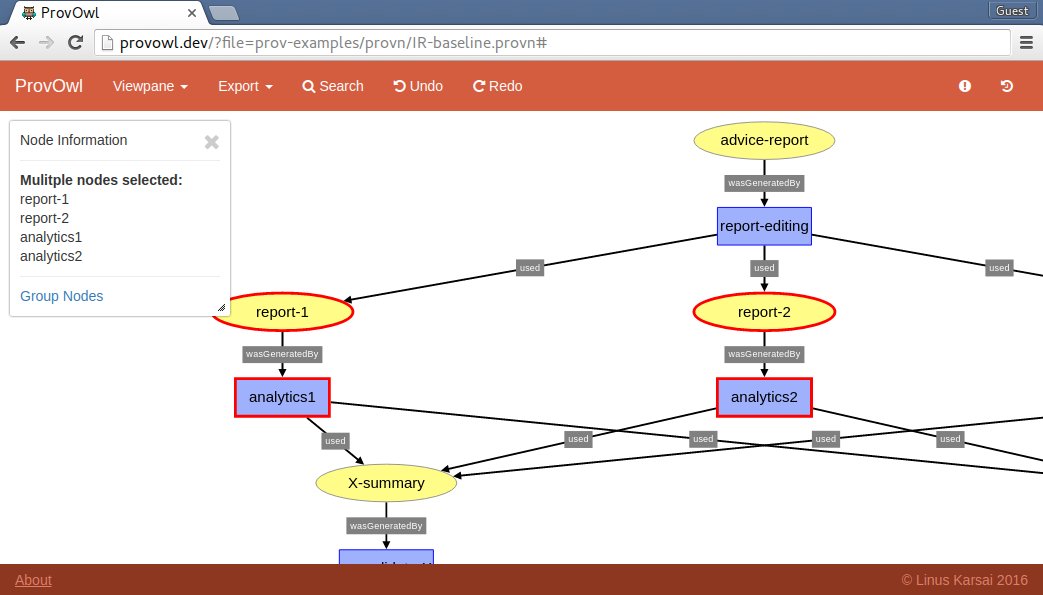
\includegraphics[width=\linewidth]{naming1}
	\caption{Using the \textit{IR-baseline} example the user has selected four nodes for grouping, essentially those related to \texttt{report-1} and \texttt{report-2}.}
	\label{fig:naming1}
\end{figure}
\begin{figure}[h]
	\centering
	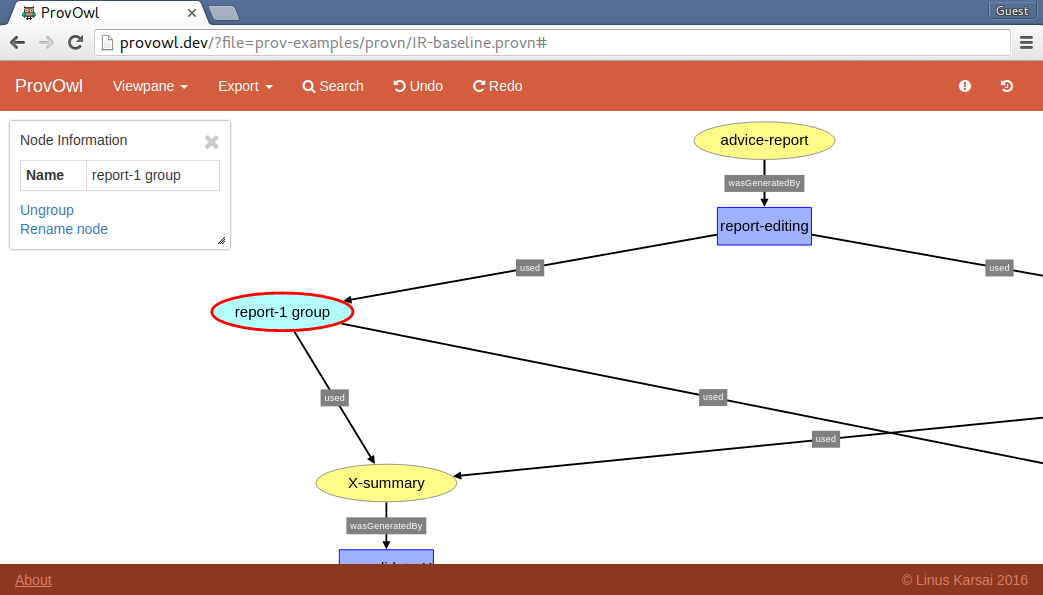
\includegraphics[width=\linewidth]{naming2}
	\caption{When clusterint the four nodes selected in Figure~\ref{fig:naming1} ProvOwl creates a composite node using the name of the node closest to the root (in this case breaking a tie by alphabetical order).}
	\label{fig:naming2}
\end{figure}
\clearpage

